\section{Техническое задание}
\subsection{Основание для разработки}

Основанием для разработки является задание выпускной квалификационной работы на создание программно-информационной системы для управления энергопотреблением в зданиях. Данная система призвана эффективно мониторить, контролировать и оптимизировать использование энергии в различных зонах зданий.

\subsection{Цель и назначение разработки}

Целью разработки программно-информационной системы является обеспечение устойчивого и эффективного управления энергопотреблением в зданиях. Основное предназначение системы — предоставление пользователю возможности контролировать, анализировать и оптимизировать расход энергии в реальном времени.

Для достижения поставленной цели необходимо решить следующие задачи:
\begin{itemize}
	\item Анализ энергетической инфраструктуры зданий, выявление ключевых факторов и паттернов потребления.
	\item Разработка концептуальной модели системы управления энергопотреблением.
	\item Проектирование программной системы, включая архитектуру, взаимодействие с устройствами и пользовательский интерфейс.
	\item Сконструирование и тестирование программной системы для управления энергопотреблением в зданиях.
\end{itemize}

\subsection{Требования пользователя к интерфейсу программной системы}

Программная система должна обеспечивать удобный и интуитивно понятный интерфейс для пользователей. В интерфейсе должны быть предусмотрены следующие элементы:
\begin{itemize}
	\item Навигацию по разделам и зонам здания.
	\item Возможность авторизации для различных уровней доступа.
	\item Отображение текущего статуса энергопотребления в различных зонах.
	\item Возможность ввода параметров для настройки системы в ручном режиме.
\end{itemize}

Страница с аналитикой энергопотребления в здании представлена на рисунках ~\ref{templ1:image} - ~\ref{templ2:image}.

%Концептуальная модель данных программной системы в виде UML-диаграммы сущность-связь представлена на рисунках ~\ref{comp1:image} - ~\ref{comp2:image}.
 
Концептуальная модель данных программной системы в виде UML-диаграммы сущность-связь представлена на рисунке ~\ref{comp:image}.

\begin{figure}[ht]
\center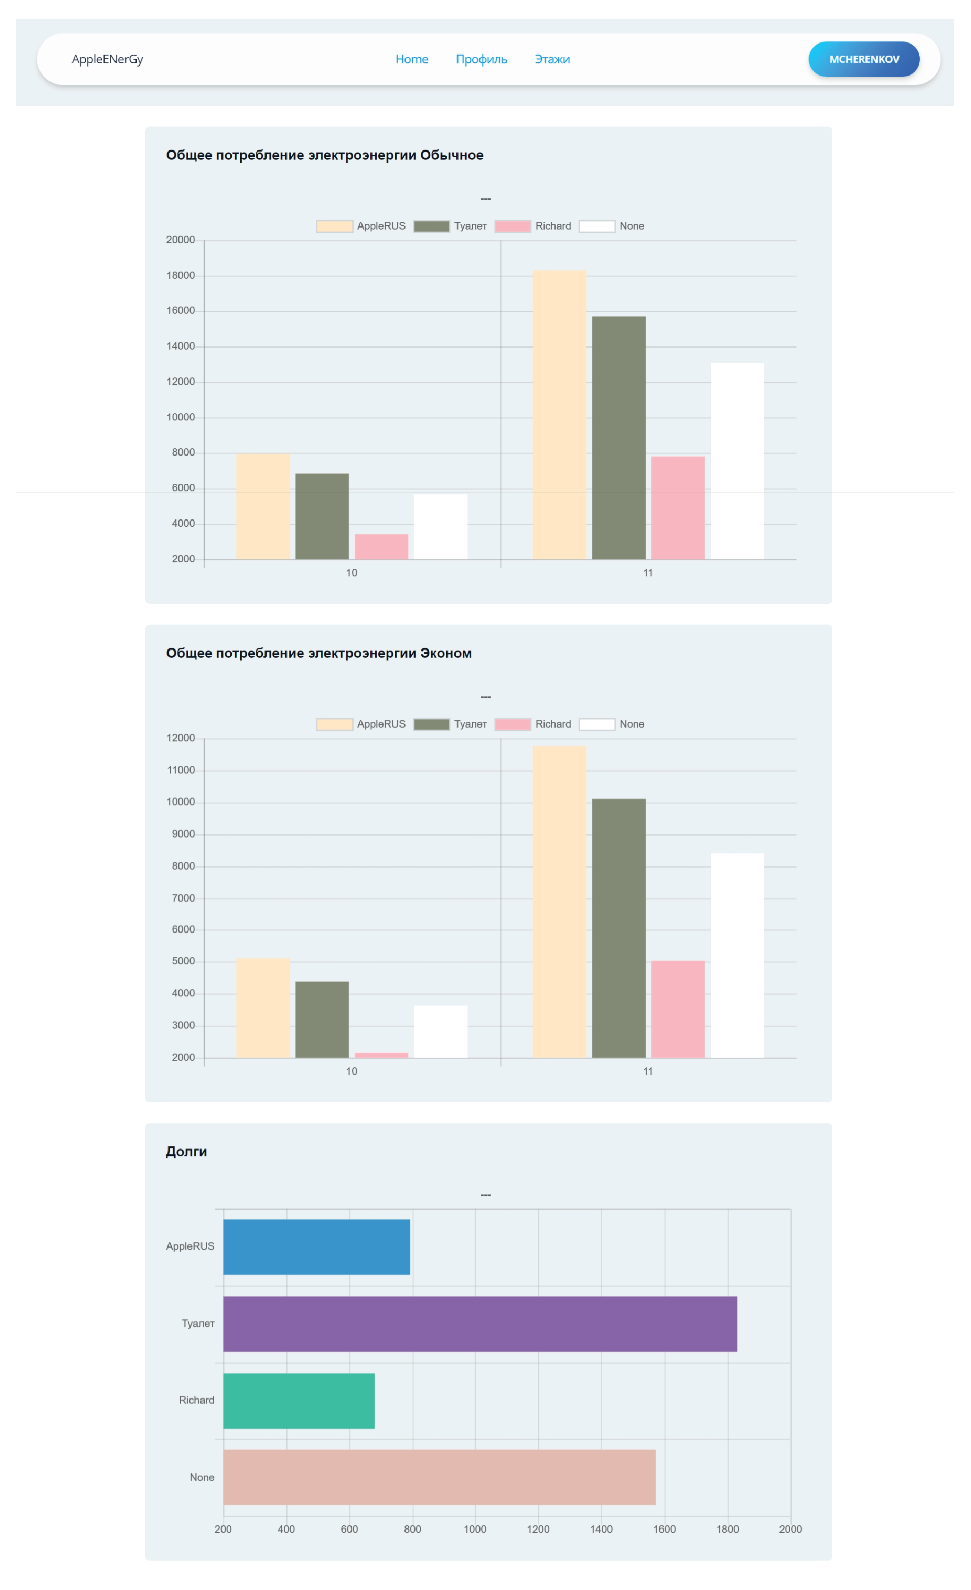
\includegraphics[width=0.65\linewidth]{templ1}
\caption{Страница с аналитикой энергопотребления в здании}
\label{templ1:image}
\end{figure}

\newpage % при необходимости можно переносить рисунок на новую страницу

\begin{figure}[ht]
	\center\includegraphics[width=0.75\linewidth]{templ2}
	\caption{Страница с аналитикой энергопотребления в здании}
	\label{templ2:image}
\end{figure}

\newpage % при необходимости можно переносить рисунок на новую страницу

\begin{figure}[ht]
	\center\includegraphics[width=0.89\linewidth]{comp}
	\caption{Концептуальная модель данных}
	\label{comp:image}
\end{figure}

%\begin{figure}[ht]
%	\includegraphics[width=1\linewidth]{comp1}
%	\caption{Концептуальная модель данных}
%	\label{comp1:image}
%\end{figure}

%\begin{figure}[ht]
%	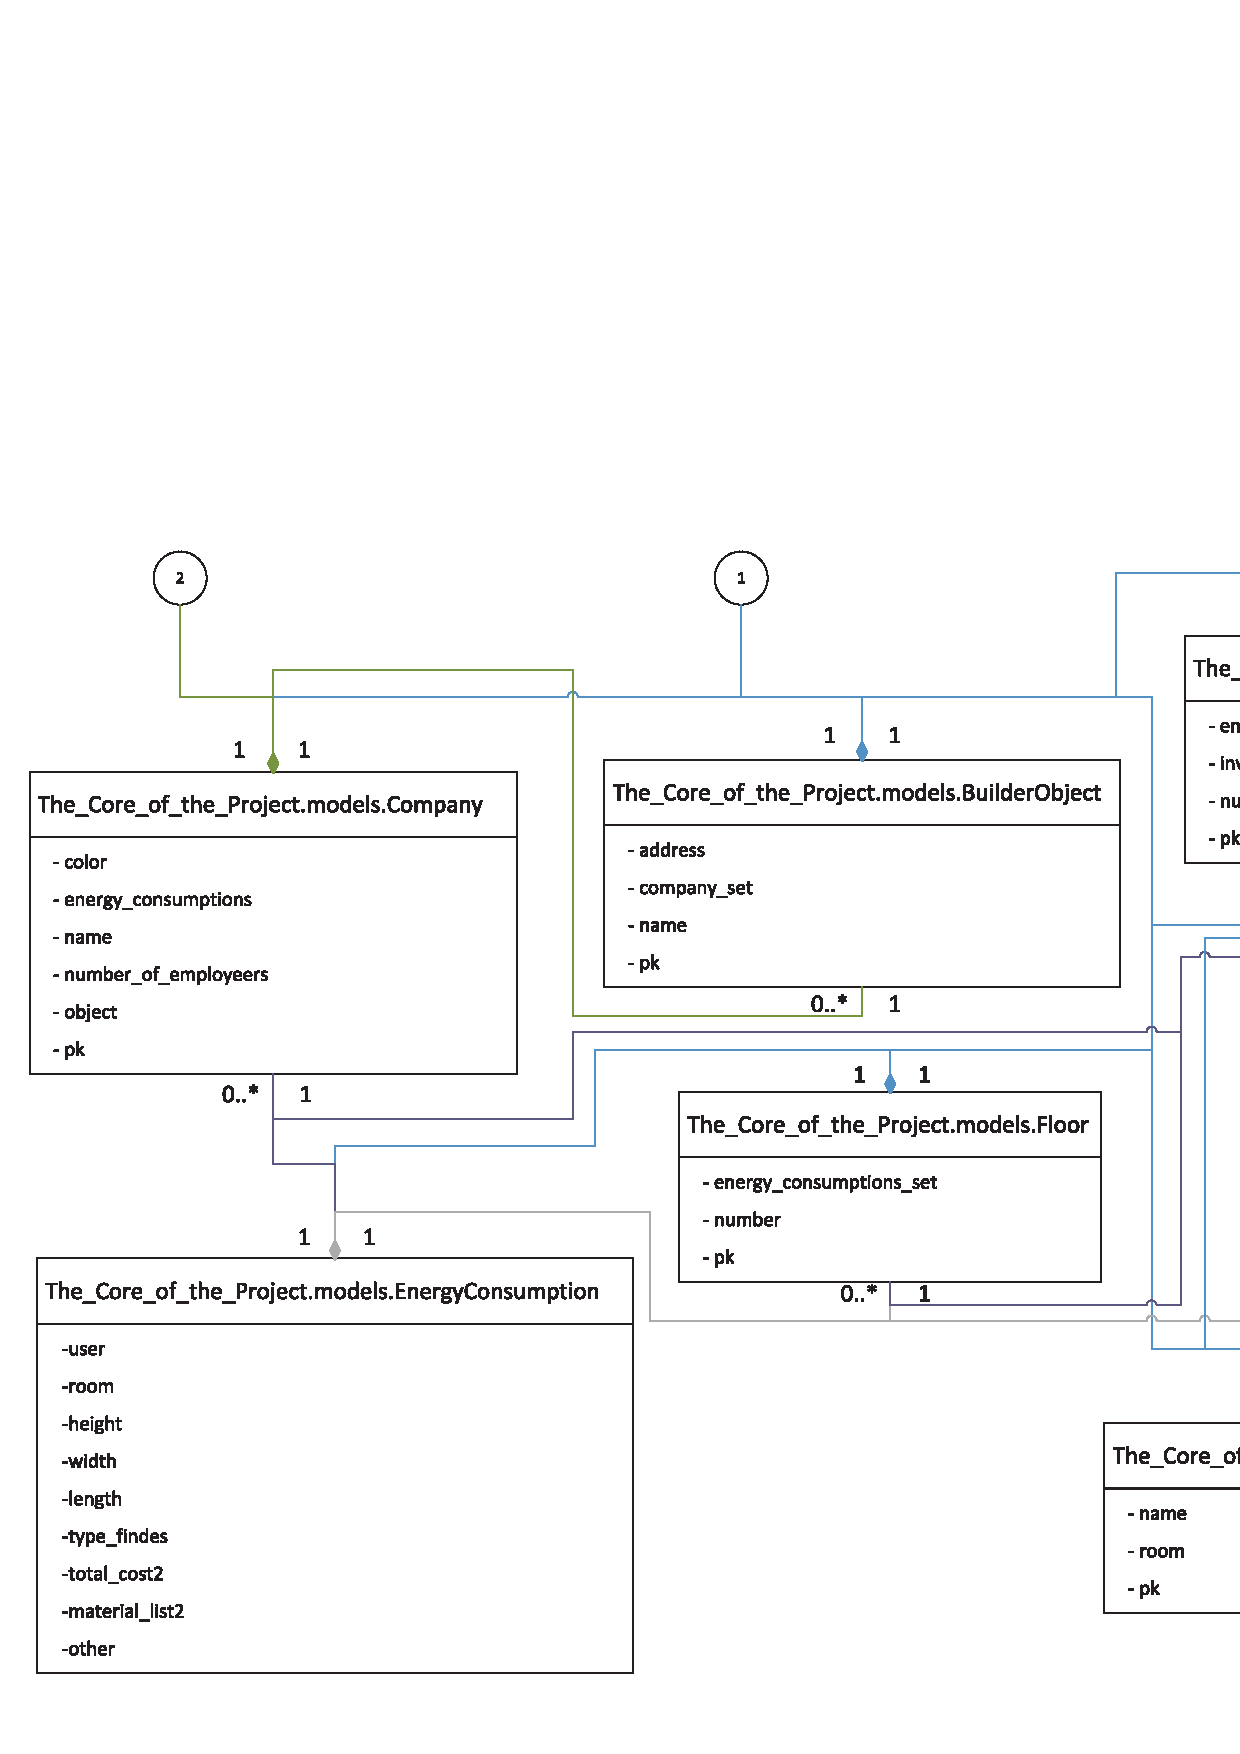
\includegraphics[width=1\linewidth]{comp2}
%	\caption{Концептуальная модель данных}
%	\label{comp2:image}
%\end{figure}

Для обеспечения удобства использования программной системы и удовлетворения потребностей пользователя, определены следующие требования к интерфейсу.

\textbf{Входные данные}

{Показания с датчиков:} Пользователь может вводить информацию о потреблении энергии вручную или автоматически, полученную от датчиков в помещениях компаний. Эти данные включают в себя значения потребления электроэнергии с и без использования умного помощника, общее количество потребляемой электроэнергии, общую стоимость потребления и данные о влажности, температуре, освещенности и наличии движения.

{Информация о помещениях, компаниях и других сущностях:} Для корректного анализа данных необходимо вводить информацию о помещениях, компаниях, этажах, предметах инвентаризации и ценах на электроэнергию.

\textbf{Выходные данные}

{Отчеты и аналитика:} Система предоставляет пользователю различные отчеты и аналитическую информацию о потреблении энергии компаниями. Эти данные включают в себя статистику по потреблению, расходам, влажности, температуре, освещенности и движению.

{Графики и визуализация:} Для наглядного представления данных система предоставляет графики и визуализацию, позволяя пользователю легко интерпретировать информацию.

{Управление данными:} Пользователь может вносить изменения в информацию о помещениях, компаниях и других сущностях через интерфейс системы.

{Оповещения:} В случае выявления аномалий или превышения установленных пороговых значений, система предоставляет уведомления и оповещения пользователю.

Система должна обеспечивать простоту ввода данных, интуитивно понятный интерфейс для взаимодействия с аналитикой, а также обеспечивать возможность быстрого доступа к ключевой информации о потреблении энергии.


%\vspace{-\figureaboveskip} % двойной отступ не нужен (можно использовать, если раздел заканчивается картинкой)

\subsection{Моделирование вариантов использования}

Для проектирования программной системы была создана модель вариантов использования. Данная модель представляет собой набор сценариев взаимодействия пользователей с системой. Диаграмма прецедентов представлена на рисунке ~\ref{precedent:image}. Она включает следующие прецеденты:

\begin{figure}[ht]
	\includegraphics[width=1\linewidth]{precedent}
	\caption{Диаграмма прецедентов}
	\label{precedent:image}
\end{figure}

{Пользовательские прецеденты:}

{\textbf{Мониторинг энергопотребления}}

\textit{Описание:} Пользователь, будучи администратором, может просматривать текущий статус энергопотребления в различных зонах здания. Эта функциональность предоставляет наглядное представление о расходе энергии и помогает выявить потенциальные проблемы.

\textit{Включает:} 
\begin{itemize}
	\item Просмотр статуса энергопотребления по зонам.
	\item Отображение графиков и диаграмм энергопотребления.
\end{itemize}

{\textbf{Настройка параметров}}

\textit{Описание:} Пользователь, имеющий права администратора, может вносить изменения в параметры системы. Это включает в себя настройку пороговых значений, оптимизацию работы системы в соответствии с текущей потребностью, и внесение изменений в режим работы оборудования.

\textit{Включает:} 
\begin{itemize}
	\item Установка пороговых значений энергопотребления.
	\item Активация/деактивация режимов работы оборудования.
	\item Регулирование параметров оптимизации энергопотребления.
\end{itemize}

{\textbf{Отчеты и аналитика}}

\textit{Описание:} Администратор системы может генерировать отчеты и аналитическую информацию о энергопотреблении. Эти отчеты предоставляют детальную статистику, позволяющую анализировать эффективность системы и выявлять тренды в потреблении энергии.

\textit{Включает:} 
\begin{itemize}
	\item Генерация отчетов по энергопотреблению за определенный период времени.
	\item Просмотр статистики по различным зонам и устройствам.
	\item Анализ трендов и предоставление рекомендаций для оптимизации.
\end{itemize}

{Системные прецеденты:}

{\textbf{Интеграция с устройствами}}

\textit{Описание:} Система должна взаимодействовать с устройствами, измеряющими энергопотребление в здании. Это включает в себя подключение к датчикам, извлечение данных и передачу команд для управления оборудованием.

\textit{Включает:} 
\begin{itemize}
	\item Подключение к датчикам энергопотребления.
	\item Извлечение данных о текущем энергопотреблении.
	\item Передача команд для регулирования работы оборудования.
\end{itemize}

{\textbf{Обработка данных}}

\textit{Описание:} Система должна обрабатывать данные, полученные от устройств, проводить анализ и формировать статистику для дальнейшего использования. Это включает в себя фильтрацию данных, выявление аномалий и расчет ключевых показателей энергопотребления.

\textit{Включает:} 
\begin{itemize}
	\item Фильтрация и агрегация данных от устройств.
	\
	
	item Анализ энергопотребления для выявления аномалий.
	\item Расчет статистических показателей для формирования отчетов.
\end{itemize}

{\textbf{Управление системой}}

\textit{Описание:} Администратор системы должен иметь возможность управлять работой системы, в том числе изменять параметры, добавлять новые устройства, и обеспечивать непрерывную работу программно-информационной системы.

\textit{Включает:} 
\begin{itemize}
	\item Добавление и удаление устройств в системе.
	\item Регулирование параметров системы для оптимальной работы.
	\item Обеспечение непрерывной работы системы и решение возможных проблем.
\end{itemize}



\subsubsection{Вариант использования <<Регистрация пользователя>>}

Заинтересованные лица и их требования: Пользователь, который не имеет учетной записи в системе, желает создать новый аккаунт.

Предусловие: Пользователь не авторизован в системе.

Постусловие: У пользователя создана учетная запись в системе.

Основной успешный сценарий:
\begin{itemize}
\item Пользователь открывает страницу регистрации.
\item Вводит свои персональные данные, такие как имя, адрес электронной почты, и пароль.
\item Нажимает кнопку "Зарегистрироваться".
\item Система проверяет валидность введенных данных.
\item В случае успешной валидации, система создает новую учетную запись пользователя.
\item Пользователю отправляется подтверждение регистрации на указанный адрес электронной почты.
\end{itemize}


\subsubsection{Вариант использования <<Регистрация компании>>}

Заинтересованные лица и их требования: Представитель компании, которая не имеет учетной записи в системе, желает зарегистрировать компанию для использования функционала системы.

Предусловие: Представитель компании не авторизован в системе.

Постусловие: В системе создана учетная запись компании, и ей назначен уникальный идентификатор.

Основной успешный сценарий:
\begin{itemize}
	\item Представитель компании открывает страницу регистрации компании.
	\item Вводит данные о компании, такие как название, цвет, расположение и количество сотрудников.
	\item Нажимает кнопку "Зарегистрировать компанию".
	\item Система проверяет валидность введенных данных.
	\item В случае успешной валидации, система создает новую учетную запись компании и присваивает ей уникальный идентификатор.
	\item Представителю компании отправляется подтверждение регистрации компании.
\end{itemize}

\subsubsection{Вариант использования <<Добавление помещения>>}

Заинтересованные лица и их требования: Пользователь (администратор), который авторизован в системе и желает добавить информацию о новом помещении.

Предусловие: Пользователь авторизован в системе и имеет доступ к функционалу управления помещениями.

Постусловие: В системе добавлена информация о новом помещении.

Основной успешный сценарий:
\begin{itemize}
	\item Пользователь переходит на страницу управления помещениями.
	\item Нажимает кнопку "Добавить помещение".
	\item Заполняет необходимые атрибуты помещения, такие как номер, площадь, этаж и прочие.
	\item Нажимает кнопку "Сохранить".
	\item Система проверяет валидность введенных данных.
	\item В случае успешной валидации, система добавляет новую информацию о помещении.
\end{itemize}

\subsubsection{Вариант использования <<Просмотр статистики по компании>>}

Заинтересованные лица и их требования: Пользователь (администратор, представитель компании), который авторизован в системе и желает получить статистическую информацию по энергопотреблению компании.

Предусловие: Пользователь авторизован в системе и имеет доступ к функционалу просмотра статистики.

Постусловие: Пользователь видит статистическую информацию по энергопотреблению компании.

Основной успешный сценарий:
\begin{itemize}
	\item Пользователь переходит на страницу статистики компании.
	\item Выбирает период, за который требуется получить статистику (например, за последний месяц).
	\item Система загружает и отображает данные о потреблении энергии компанией за выбранный период.
	\item Пользователь видит графики и диаграммы, отражающие энергопотребление, расходы и другие показатели.
\end{itemize}

\subsubsection{Вариант использования <<Просмотр статистики помещения>>}

Заинтересованные лица и их требования: Пользователь (администратор, представитель компании), который авторизован в системе и желает получить статистическую информацию по энергопотреблению определенного помещения.

Предусловие: Пользователь авторизован в системе, имеет доступ к функционалу просмотра статистики помещений и выбрал конкретное помещение.

Постусловие: Пользователь видит статистическую информацию по энергопотреблению выбранного помещения.

Основной успешный сценарий:
\begin{itemize}
	\item Пользователь переходит на страницу статистики помещения.
	\item Выбирает период, за который требуется получить статистику (например, за последний месяц).
	\item Система загружает и отображает данные о потреблении энергии выбранным помещением за выбранный период.
	\item Пользователь видит графики и диаграммы, отражающие энергопотребление, расходы и другие показатели для данного помещения.
\end{itemize}


\subsubsection{Вариант использования <<Добавление устройства>>}

Заинтересованные лица и их требования: Пользователь (администратор), который авторизован в системе и желает добавить информацию об устройстве, подключенном к определенному помещению.

Предусловие: Пользователь авторизован в системе и имеет доступ к функционалу управления устройствами помещения.

Постусловие: Информация об устройстве добавлена в систему для выбранного помещения.

Основной успешный сценарий:
\begin{itemize}
	\item Пользователь переходит на страницу управления устройствами для конкретного помещения.
	\item Выбирает опцию "Добавить устройство".
	\item Вводит информацию о новом устройстве, такую как название, тип, идентификатор, и другие характеристики.
	\item Нажимает кнопку "Добавить".
	\item Система проверяет валидность введенных данных.
	\item В случае успешной валидации, информация об устройстве добавляется к данным помещения.
	\item Пользователь видит обновленный список устройств для выбранного помещения.
\end{itemize}

\subsection{Требования к оформлению документации}

Разработка программной документации и программного изделия должна производиться согласно ГОСТ 19.102-77 и ГОСТ 34.601-90. Единая система программной документации.
